\documentclass[11pt]{article}
%\documentclass{book}
\usepackage[utf8]{inputenc}
\usepackage[T1]{fontenc}
\usepackage[french]{babel}
\usepackage[top=1.8cm, bottom=1.8cm, left=1.8cm, right=1.8cm]{geometry}
\usepackage[linktocpage,colorlinks=false]{hyperref}
\usepackage{graphicx}
\usepackage{epsfig}
\usepackage{amssymb}
\usepackage{amsmath}
\usepackage{array}
\usepackage{subfig}
\usepackage{multicol}
\usepackage{caption}
\usepackage{listings}
\usepackage{algorithm}
\usepackage{algorithmic}
\hypersetup{
    colorlinks=true,
    breaklinks=true,
    urlcolor=red,
}
\parskip=5pt

\title{\huge{\textbf Spécifications}}
\author{AYOUB Pierre, BASKEVITCH Claire, BESSAC Tristan, \\
CAUMES Clément, DELAUNAY Damien, DOUDOUH Yassin}
\date{Mercredi 18 Avril 2018}

\begin{document}

\maketitle
\vspace{20em}
\begin{center}
\includegraphics{pictures/Application.png}\end{center}
\newpage

\tableofcontents

\newpage

\section{Introduction}

Après avoir réalisé le cahier des charges concernant l'application StegX, 
l'analyse des contraintes et des besoins du client nous amène à rédiger 
les spécifications. 

Le logiciel StegX proposera de cacher des données dans des fichiers dont le
format est pris en charge par l'application (stéganographie). De plus, un
utilisateur pourra extraire les données cachées d'un fichier si ces données ont
étés cachées en utilisant notre application (stéganalyse). StegX prendra en
charge les trois algorithmes de stéganographie suivants : EOF, LSB et Metadata.

Durant l'analyse des fonctionnalités de l'application, nous avons vu qu'elle
devait gérer la manipulation de données binaires et qu’il fallait donc un
langage proche de la machine. De plus, nous devons implémenter des fonctions de
stéganographie afin de cacher des données dans des fichiers. Par conséquent, une
programmation procédurale était nécessaire. Enfin, il fallait des structures
afin de manipuler des structures de fichiers. De ce fait, nous avons choisi le
langage C pour implémenter la future application StegX. En effet, le langage C
propose une programmation procédurale, ainsi qu'un langage bas niveau proche de
la machine. Enfin, la possibilité d'écriture et de lecture de bits et d'accès
mémoire avec le langage C correspond à nos besoins. C'est donc pour toutes ces
raisons que l'équipe de conception de StegX a choisi le langage C pour
implémenter l'application. 

Après l'étude des différents modules de l'organigramme, ainsi que les informations 
qui se déplacent, nous avons établi un organigramme. 
Cet organigramme nous permettra ainsi de rédiger en détail les spécifications 
des différents modules de l'application. 

\section{Modules du produit}
\subsection{Organigramme}

\hspace{1cm}
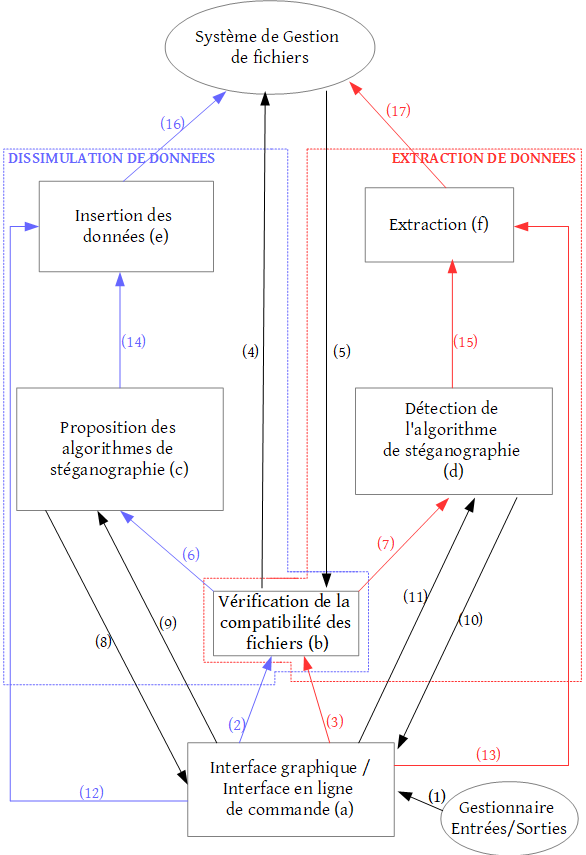
\includegraphics[scale=0.71]{pictures/organigramme.png}

\subsection{Liste des modules et de leurs fonctionnalités}

\begin{description}
\item[a)] \textbf{Interface graphique / Interface en ligne de commande} :
    interfaces permettant à l'utilisateur de choisir parmi les deux
    fonctionnalités possibles de l'application. Il peut dissimuler des
    données dans un fichier (dont le type et le format sont pris en charge
    par l'application). Ou bien, il peut extraire les données cachées d'un
    fichier. \newline
    Il aura donc un mécanisme pour choisir le fichier hôte et le fichier 
    à cacher (pour la dissimulation de données), et un mécanisme pour choisir le 
    fichier contenant les données cachées à analyser (pour l'extraction de 
    données cachées), grâce à une interaction avec le gestionnaire d’entrée/sorties. 

\item[b)] \textbf{Vérification de la compatibilité des fichiers} : le format 
	du fichier hôte (pour le module \textit{Dissimulation de données}) ou 
	le format du fichier à analyser (pour le module \textit{Extraction de données 
	cachées}), choisis par l'utilisateur, est vérifié pour savoir s'il est 
	bien pris en charge par l'application. \newline
	Il aura un mécanisme de lecture du fichier hôte : selon les formats 
	pris en charge, il y aura une série de tests successifs pour déterminer le 
	format du fichier. 
	Il prendra en entrée les chemins de fichiers en entrée. Ce module interagira
	avec le système de gestion de fichiers. 

\item[c)] \textbf{Proposition des algorithmes de stéganographie} : en fonction
    du type et du format du fichier hôte, ainsi que de la taille des données à
    cacher, un mécanisme proposera un ou plusieurs algorithmes (avec ou sans 
    sécurité supplémentaire).  

\item[d)] \textbf{Détection de l'algorithme de stéganographie} : un mécanisme 
	d'analyse du fichier permettra de découvrir quel algorithme a été utilisé 
	afin de les extraire correctement par la suite. 

\item[e)] \textbf{Insertion des données} : la copie des données du fichier hôte
    sera modifiée avec l'insertion des données à cacher à l'aide de l'algorithme
    choisi par l'utilisateur. 

\item[f)] \textbf{Extraction} : les données cachées dans le fichier à analyser
    sont extraites selon l'algorithme déduit.

\end{description}
\newpage

L'organigramme établi dans le cahier des charges représentait les informations
qui circulaient entre les modules, mais ne représentaient pas les appels de
fonctions. Pour l'implémentation de StegX, il est nécessaire que les modules
soient indépendants. Pourtant, si on interprétait l’organigramme initial comme
un organigramme d’appel de fonction, il imposerait le fait que les modules
soient dépendants. Par exemple, une fonction du module \textit{Vérification de
la compatibilité des fichiers} devait appeler une fonction du sous-module
\textit{Détection de l'algorithme de stéganographie} qui devait appeler une
autre fonction du sous-module \textit{Extraction}. Or, StegX propose une
bibliothèque et donc il faut pouvoir proposer aux développeurs qui l'utilisent
des fonctions indépendantes de chaque sous-module de dissimulation/extraction.
Par exemple, un développeur pourra juste réaliser la détection de l'algorithme
de stéganographie sur des fichiers qu'ils considèrent déjà comme vérifié. De
plus, il fallait que les interfaces (en ligne de commande et graphique)
appellent elles-mêmes chacun des modules, et non qu'un module appelle un autre. 

C'est pour cette raison que l'organigramme proposé dans les spécifications
semble plus représentatif de la future implémentation de StegX puisqu'il fait
apparaître les réels appels de fonctions. En effet, dans ce nouvel organigramme,
ce sont les interfaces qui appellent dans un ordre précis les différents
modules. Avec ce nouvel organigramme, on peut réaliser séquentiellement et
indépendamment chaque étape de la dissimulation ou de l'extraction. 

%\hspace{0.3cm}
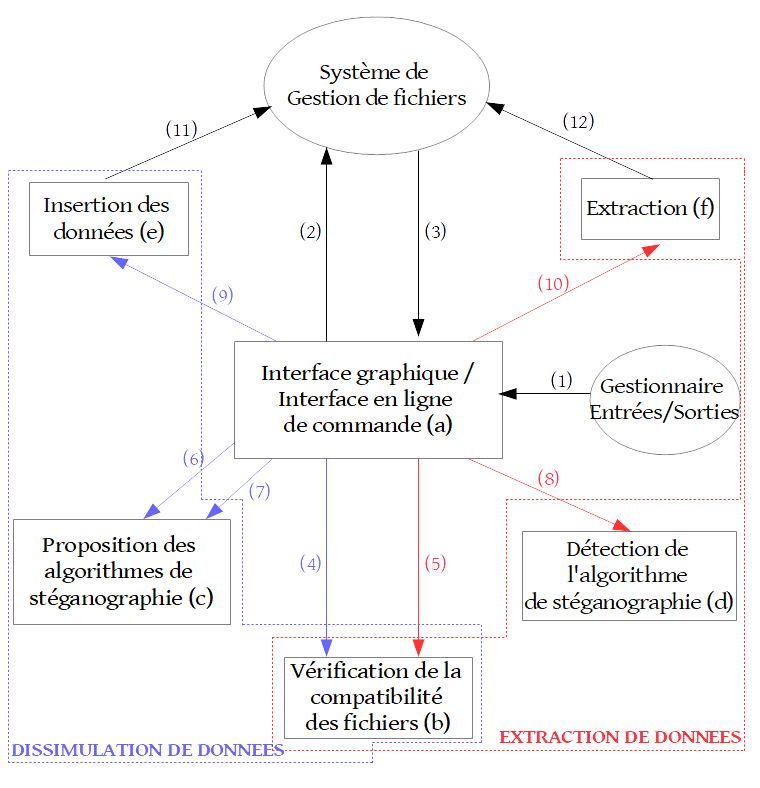
\includegraphics[scale=0.6]{pictures/organigramme2.png}
\newpage

\paragraph{Liste des informations qui circulent entre les modules :}

\begin{multicols}{2}
\begin{description}
\item[1)] %OK
\begin{itemize}
\item Utilisation de l'application (dissimulation ou extraction).
\item Mot de passe choisi par l'utilisateur. 
\item Nom du fichier hôte, nom du fichier à cacher et chemin du fichier à créer
    (pour la dissimulation).
\item Nom du fichier à analyser et chemin du fichier résultant de l'extraction
    des données cachées (pour l'extraction).
\end{itemize}
\item[2)]  %OK
\begin{itemize}
\item Nom du fichier hôte et nom du fichier à cacher (pour la dissimulation).
\item Nom du fichier contenant les données cachées à analyser (pour l'extraction).
\end{itemize}
\item[3)] %OK
\begin{itemize}
\item Fichier hôte et fichier à cacher (pour la dissimulation). 
\item Fichier contenant les données cachées à analyser (pour l'extraction). 
\end{itemize}
\item[4)] %OK
\begin{itemize}
\item Fichier hôte dont il faut vérifier la compatibilité. 
\end{itemize}
\item[5)] %OK
\begin{itemize}
\item Fichier à analyser dont il faut vérifier la compatibilité.
\end{itemize}
\item[6)] %OK
\begin{itemize}
\item Fichier hôte.
\item Fichier à cacher.
\end{itemize}
\item[7)] %OK
\begin{itemize}
\item Algorithme choisi par l'utilisateur. 
\end{itemize}
\item[8)] %OK
\begin{itemize}
\item Fichier à analyser dont il faut détecter l'algorithme utilisé. 
\item Mot de passe choisi par l'utilisateur. 
\end{itemize}
\item[9)] %OK
\begin{itemize}
\item Fichier hôte. 
\item Fichier à cacher. 
\item Algorithme à utiliser. 
\item Mot de passe choisi par l'utilisateur. 
\item Fichier résultant (dans lequel il faut écrire). 
\end{itemize}
\item[10)] %OK
\begin{itemize}
\item Fichier à analyser.
\item Algorithme détecté. 
\item Mot de passe choisi par l'utilisateur. 
\item Fichier à créer (lors de l'extraction). 
\end{itemize}
\item[11)] 
\begin{itemize}
\item Écriture du fichier à créer qui dissimulera les données à cacher et aura
    l'apparence du fichier hôte.
\end{itemize}
\item[12)]
\begin{itemize}
\item Écriture du fichier extrait qui était caché dans le fichier hôte.
\end{itemize}
\end{description}
  \ldots
\end{multicols}

\paragraph{Détails d'un déroulement d'utilisation de l'application pour la 
dissimulation}

\begin{itemize}
\item Phase 1 : Récupération des entrées de l'utilisateur : (1)
\item Phase 2 : Initialisation, ouverture des fichiers et test de la 
validité des fichiers en entrée : (2) et (3)
\item Phase 3 : Vérification de la compatibilité du fichier hôte : (4)
\item Phase 4 : Proposition des algorithmes selon les entrées de départ : 
(6)
\item Phase 5 : Choix de l'algorithme selon la proposition des algorithmes : 
(7)
\item Phase 6 : Insertion des données : (9) et (11)
\end{itemize}

\paragraph{Détails d'un déroulement d'utilisation de l'application pour 
l'extraction}

\begin{itemize}
\item Phase 1 : Récupération des entrées de l'utilisateur : (1)
\item Phase 2 : Initialisation, ouverture des fichiers et test de la 
validité des fichiers en entrée : (2) et (3)
\item Phase 3 : Vérification de la compatibilité du fichier à analyser : 
(5)
\item Phase 4 : Détection de l'algorithme utilisé : (8)
\item Phase 5 : Extraction : (10) et (12)
\end{itemize}
\newpage

\section{Description des structures de données}

\subsection{Description des énumérations}

\begin{lstlisting}[language=c]
enum mode {STEGX_MODE_INSERT, STEGX_MODE_EXTRACT};
typedef enum mode mode_e;
\end{lstlisting}

L'énumération mode permet de distinguer les deux outils proposés par 
l'application : extraire ou dissimuler. 
\newline

\begin{lstlisting}[language=c]
enum algo {STEGX_ALGO_LSB, STEGX_ALGO_EOF, STEGX_ALGO_METADATA, 
        STEGX_ALGO_EOC, STEGX_ALGO_JUNK_CHUNK};
typedef enum algo algo_e;
\end{lstlisting}

L'énumération \textit{algo} distingue les différents algorithmes proposés par 
l'application. 
Les énumérations \textit{STEGX\_ALGO\_EOC} pour le format \textit{FLV} et
\textit{STEGX\_ALGO\_JUNK\_CHUNK} pour les formats \textit{AVI} concernent 
deux algorithmes supplémentaires. Ces algorithmes n'ont pas été détaillés 
dans le cahier des charges et ne seront implémentés qu'en supplément, si 
les concepteurs ont le temps avant de rendre l'application finale. 

Le format \textit{FLV} est divisé en 3 sortes de "tags" : vidéo, audio et 
data. L'algorithme \textit{EOC} consiste à écrire après chaque tag vidéo 
qu'on appelle "chunk". Ainsi, les données écrites après ces chunks ne seront 
pas interprétées. 

Dans le format \textit{AVI}, il existe une sorte de chunk "poubelle" (junk) 
qui permet d'écrire n'importe quelle donnée et qui ne sera pas interprété
par le lecteur. Le principe de l'algorithme \textit{Junk Chunk} est de créer 
un ou plusieurs junk chunks et de cacher les données dedans. 
\newline 

\begin{lstlisting}[language=c]
enum type {BMP_COMPRESSED, BMP_UNCOMPRESSED, PNG, WAV_PCM, WAV_NO_PCM, 
        MP3, AVI_COMPRESSED, AVI_UNCOMPRESSED, FLV, UNKNOWN};
typedef enum type type_e;
\end{lstlisting}

L'énumération \textit{type} expose les différents formats de fichiers avec leurs 
particularités pour certains. Si le format du fichier hôte ou à analyser 
est inconnu, cela sera représenté par le type UNKNOWN. \newline


\begin{lstlisting}[language=c]
enum method {STEGX_WITHOUT_PASSWD, STEGX_WITH_PASSWD};
typedef enum method method_e;
\end{lstlisting}

L'énumération \textit{method} permettra de connaître si l'utilisateur choisit
d'utiliser la méthode de protection des données ou non. \newline

\subsection{Description des structures}

\begin{lstlisting}[language=c]
struct stegx_info_insert {
    char* hidden_path;
    algo_e algo;
};
typedef struct stegx_info_insert stegx_info_insert_s;
\end{lstlisting}

La structure stegx\_info\_ins permet de représenter les informations 
nécessaires sur le fichier à cacher, c'est-à-dire son chemin et l'algorithme que 
l'on utilisera pour dissimuler ce dernier. \newline
\underline{Paramètres :}
\begin{itemize}
\item \textit{hidden\_path} est une chaine de caractères représentant le nom du fichier 
à cacher. 
\item \textit{algo} représente l'algorithme qui sera utilisé pour dissimuler. 
\newline
\end{itemize}

\begin{lstlisting}[language=c]
struct stegx_choices {
    char* host_path;
    char* res_path;                         
    char* passwd;                           
    mode_e mode;                        
    stegx_info_insert_s* insert_info;             
};
typedef struct stegx_choices stegx_choices_s;
\end{lstlisting}

La structure stegx\_choices représente les données choisies par l'utilisateur 
s'il veut dissimuler ou extraire des données. \newline
\underline{Paramètres :}
\begin{itemize}
\item \textit{host\_path} est une chaine de caractères représentant le chemin
du fichier à analyser (pour l'extraction) ou hôte (pour la dissimulation). 
\item \textit{res\_path} est une chaine de caractères représentant le chemin
du fichier résultant (pour l'extraction ou pour la dissimulation). 
\item \textit{passwd} est une chaine de caractères représentant le mot de passe 
choisi par l'utilisateur. Celui-ci est optionnel et si l'utilisateur choisit 
de ne pas en mettre, passwd vaudra NULL. 
\item \textit{mode} est une variable d'énumération représentant le mode que 
l'utilisateur a choisi : dissimulation (STEGX\_MODE\_INSERT)ou extraction 
(STEGX\_MODE\_EXTRACT).  
\item \textit{* ins\_info} est un pointeur sur la structure stockant les informations 
sur le fichier à cacher. Elle est requise si le champ mode est à STEGX\_MODE\_INSERT. 
\newline
\end{itemize}

\begin{lstlisting}[language=c]
struct host_info {
    FILE* host;
    type_e type;
    union {
        struct bmp bmp;
        struct png png;
        struct wav wav;
        struct mp3 mp3;
        struct avi avi;
        struct flv flv;
    } file_info;
};
typedef struct host_info host_info_s;
\end{lstlisting}

Cette structure host\_info permet de stocker les informations 
utiles pour chaque format différent afin de le manipuler convenablement 
par la suite. 
\newline
\underline{Paramètres :}
\begin{itemize}
\item \textit{host} représente le fichier hôte pour le cas de la dissimulation 
et le fichier à analyser pour le cas de l'extraction. 
\item \textit{type} permet de distinguer quel champ il faut manipuler pour l'union 
\textit{infos}. Pour chaque format, il y un ou plusieurs types possibles.
\item \textit{file\_info} est une union en C. Elle permet de choisir un champ parmi
ceux qui sont définis. Ainsi, si le fichier hôte est un fichier BMP par exemple, 
seule la structure bmp de infos sera initialisée et manipulée par la suite.
\newline
\end{itemize}

\begin{lstlisting}[language=c]
struct bmp {
    uint32_t header_size;
    uint32_t data_size;
    uint32_t pixel_number;
    uint32_t pixel_size;
};
typedef struct bmp bmp_s;
\end{lstlisting}

La structure \textit{bmp\_s} correspond aux informations 
utiles pour le format BMP.  
\newline
\underline{Paramètres :}
\begin{itemize}
\item \textit{header\_size} représente la taille du header (contenant les 
informations pour interpréter correctement un fichier BMP), soit l'octet 
du début des données brutes. 
\item \textit{data\_size} représente la taille en octets des données brutes 
(représenté ici par des composantes de pixels). On aura donc 
\textit{[taille fichier]} = \textit{header\_size} + \textit{data\_size}.
\item \textit{pixel\_number} représente le nombre de bits par pixel. 
\item \textit{pixel\_size} représente le nombre de pixels dans l'image BMP. 
\newline
\end{itemize}

\begin{lstlisting}[language=c]
struct png {
    uint32_t header_size;
    uint32_t data_size;
};
typedef struct png png_s;
\end{lstlisting}

La structure \textit{png\_s} correspond aux informations 
utiles pour le format PNG.  
\newline
\underline{Paramètres :}
\begin{itemize}
\item \textit{header\_size} représente la taille du header (contenant les 
informations pour interpréter correctement un fichier PNG), soit l'octet 
du début des données représentant l'image réelle. 
\item \textit{data\_size} représente la taille en octets des données compressées. 
On aura donc 
\textit{[taille fichier]} = \textit{header\_size} + \textit{data\_size}.
\newline
\end{itemize}

\begin{lstlisting}[language=c]
struct wav {
    uint32_t header_size;
    uint32_t data_size;
    uint32_t chunk_size;
};
typedef struct wav wav_s;
\end{lstlisting}

La structure \textit{wav\_s} correspond aux informations 
utiles pour le format WAV.  
\newline
\underline{Paramètres :}
\begin{itemize}
\item \textit{header\_size} représente la taille du header (contenant les 
informations pour interpréter correctement un fichier WAV), soit l'octet 
du début des données brutes. 
\item \textit{data\_size} représente la taille en octets des données brutes 
(représenté ici par du son). On aura donc 
\textit{[taille fichier]} = \textit{header\_size} + \textit{data\_size}.
\item \textit{chunk\_size} représente le nombre de bits par sample (échantillon 
de son). 
\newline
\end{itemize}

\begin{lstlisting}[language=c]
struct mp3 {
    uint64_t sig_addr;
};
typedef struct mp3 mp3_s;
\end{lstlisting}

La structure \textit{mp3\_s} correspond aux informations 
utiles pour le format MP3.  
\newline
\underline{Paramètres :}
\begin{itemize}
\item \textit{sig\_addr} représente l'adresse absolue de la signature StegX 
présente dans le fichier hôte. 
\newline
\end{itemize}

\begin{lstlisting}[language=c]
struct avi {
    uint64_t sig_addr;
};
typedef struct avi avi_s;
\end{lstlisting}

La structure \textit{avi\_s} correspond aux informations 
utiles pour le format AVI.  
\newline
\underline{Paramètres :}
\begin{itemize}
\item \textit{sig\_addr} représente l'adresse absolue de la signature StegX 
présente dans le fichier hôte. 
\newline
\end{itemize}

\begin{lstlisting}[language=c]
struct flv {
    uint32_t nb_video_tag;
    uint32_t nb_metadata_tag;
    uint32_t file_size;
};
typedef struct flv flv_s;
\end{lstlisting}

La structure \textit{flv\_s} correspond aux informations 
utiles pour le format FLV.  
\newline
\underline{Paramètres :}
\begin{itemize}
\item \textit{nb\_video\_tag} représente le nombre de chunks de video dans 
le fichier. 
\item \textit{nb\_metadat\_tag} représente le nombre de chunks de metadonnées. 
\item \textit{file\_size} représente la taille du fichier. 
\newline
\end{itemize}

\begin{lstlisting}[language=c]
struct info {
    mode_e mode;  
    algo_e algo; 
    method_e method;            
    host_info_s host;           
    FILE* res;                 
    FILE* hidden;              
    char* hidden_name;
    int hidden_length; 
    char* passwd;
};
typedef struct info info_s;
\end{lstlisting}

La structure info correspond à la structure interne à la bibliothèque :
elle va contenir toutes les informations utiles pour la dissimulation ou 
l'extraction des données. 
\newline
\underline{Paramètres :}
\begin{itemize}
\item \textit{mode} est une variable d'énumération représentant le mode que 
l'utilisateur a choisi : dissimulation (STEGX\_MODE\_INSERT)ou extraction 
(STEGX\_MODE\_EXTRACT). 
\item \textit{algo} est l'énumération représentant l'algorithme qui sera utilisé
pour la dissimulation ou l'extraction. 
\item \textit{method} est la variable permettant de savoir si l'utilisateur 
a choisi la méthode de protection des données. 
\item \textit{host} va contenir le détail du fichier hôte pour le bon déroulement 
de la dissimulation/extraction (selon les cas d'utilisation). 
\item \textit{res} représente le fichier résultat qui va être créé pour la 
dissimulation ou l'extraction.  
\item \textit{hidden} représente le fichier à cacher dans le cas de l'insertion. 
Il est donc requis si mode vaut STEGX\_MODE\_INSERT. 
\item \textit{hidden\_name} représente le nom du fichier à cacher/caché selon 
les cas. 
\item \textit{hidden\_length} représente la taille du fichier à cacher/caché. 
Cette information est nécessaire dans l'extraction pour connaitre combien de 
données il reste à extraire dans le fichier. Dans la dissimulation, ce champ 
permet de construire correctement les informations globales du fichier caché. 
\item \textit{passwd} est la chaine de caractères représentant le mot de passe 
choisi par l'utilisateur. 
\newline
\end{itemize}

\section{Description des différents modules}
\subsection{Interface graphique}

L'interface graphique permettra à un utilisateur de manipuler correctement
l'application StegX. Ainsi, un utilisateur non initié à l'informatique pourra
facilement utiliser notre l'application. 

Dans le cadre du développement de notre logiciel, nous privilégions les
solutions multiplate-formes et libres. L'idéal serait donc une bibliothèque
graphique remplissant ces critères, en plus d'être relativement haut niveau et
utilisable en C. De nombreuses bibliothèques graphiques proposent de tels
fonctionnalités, par exemple Qt, GTK+, wxWidgets pour ne citer qu'eux. Lors de
notre précédent projet, nous avions déjà appris à utiliser Qt. Nous souhaitions
dès lors apprendre à utiliser une nouvelle bibliothèque plutôt que nous baser
sur nos acquis, nous avons donc opté pour GTK+ qui correspondait à tout notre
critères.

GTK+ est une bibliothèque graphique libre, multiplate-forme, développée à
l'origine pour le logiciel de traitement d'image GIMP. Très utilisée dans
l'environnent de bureau GNOME, cette bibliothèque propose un large panel de
fonctionnalité, dont le paradigme des widgets pour la création de l'interface et
celui des signaux pour la gestion de l'interaction avec l'utilisateur.
Travailler avec GTK+ nous permettra de nous familiariser avec l'environnent et
les bibliothèques utilisés par GNOME et GTK+, à savoir GDK, GLib, GIO et
GObject.

Pour écrire ces spécifications, nous avons donc eu à étudier quels widgets
seront utilisés, ainsi que les signaux à mettre en oeuvre pour mettre en
relation ces derniers avec les actions de l'utilisateur. Dans le but de stocker
les informations de l'interface utilisateur, nous allons créer une structure
nommée \textit{struct ui} qui contiendra tous les widgets utilisés dans
l'interface ainsi que les différents messages affichés par le programme. De
plus, l’interface graphique agira comme une machine à état pour l’insertion. En
effet, il faut différencier l'état où l’utilisateur doit d’abord lancer
l’analyse des fichiers et celui où il peut lancer la dissimulation.

\begin{lstlisting}[language=c]
void ui_create (GtkWidget* window, struct ui* ui);
\end{lstlisting}

Cette fonction va permettre de créer entièrement l'interface utilisateur 
sur une fenêtre donnée. Elle construira les widgets et configure les signaux. 
\newline
\underline{Entrées :} 
\begin{itemize}
\item \textit{*window :} pointeur vers la fenêtre sur laquelle construire 
l'interface utilisateur. 
\item \textit{*ui :} pointeur vers l'interface utilisateur à remplir. 
\newline 
\end{itemize}

\begin{lstlisting}[language=c]
void ui_build (struct ui* ui);
\end{lstlisting}

Cette fonction va construire la fenêtre principale en ajoutant les conteneurs 
et les widgets. 
\newline
\underline{Entrée :} 
\begin{itemize}
\item \textit{*ui :} pointeur vers l'interface utilisateur où il faut construire 
l'affichage. 
\newline 
\end{itemize}

\begin{lstlisting}[language=c]
void ui_signal_init (struct ui* ui);
\end{lstlisting}

Cette fonction va initialiser les signaux et connecter ces derniers aux 
widgets de la fenêtre principale. 
\newline
\underline{Entrée :} 
\begin{itemize}
\item \textit{*ui :} pointeur vers l'interface utilisateur où il faut 
configurer les signaux. 
\newline 
\end{itemize}
 
\begin{lstlisting}[language=c]
static gboolean insert_do(gpointer data);
\end{lstlisting}
Exécute l'analyse des fichiers entrés par l'utilisateur ou l'insertion des
données du fichier caché dans le fichier hôte. Met à jour une variable avec
le code de retour du traitement.
\newline
\underline{Entrée :} 
\begin{itemize}
\item \textit{gpointer data :} structure de l'interface utilisateur. 
\end{itemize}
\underline{Sortie :}
\begin{itemize}
\item \textit{gboolean :} code de retour du thread GTK+.
\newline 
\end{itemize}

\begin{lstlisting}[language=c]
static gboolean extrac_do(gpointer data);
\end{lstlisting}
Exécute l'extraction des données du fichier caché dans le fichier hôte. Met à
jour une variable avec le code de retour de l'extraction.
\newline
\underline{Entrée :} 
\begin{itemize}
\item \textit{gpointer data :} structure de l'interface utilisateur. 
\end{itemize}
\underline{Sortie :}
\begin{itemize}
\item \textit{gboolean :} code de retour du thread GTK+.
\newline 
\end{itemize}

\subsection{Interface en ligne de commande}

Concernant l'interface en ligne de commande, c'est le deuxième moyen pour 
manipuler l'application StegX. Les utilisateurs savant manipuler le terminal 
peuvent ainsi faire de la stéganographie. 

\begin{lstlisting}[language=c]
stegx_choices_s* init_choices ();
\end{lstlisting}

Cette fonction va initialiser la structure contenant les informations 
entrées en ligne de commande. 
\newline
\underline{Sortie :} 
\begin{itemize}
\item \textit{stegx\_choices\_s:} renvoie la structure initialisée. 
\newline 
\end{itemize}

\begin{lstlisting}[language=c]
void fill_info (stegx_choices_s* com, const int argc, char* const* argv);
\end{lstlisting}

La fonction va remplir la structure avec les informations entrées en 
ligne de commande. 
\newline
\underline{Entrées :} 
\begin{itemize}
\item \textit{*com :} pointeur sur la structure contenant les informations 
entrées par l'utilisateur. 
\item \textit{argc :} nombre d'arguments entrés en ligne de commande. 
\item \textit{argv :} arguments entrés en ligne de commande. 
\newline 
\end{itemize}

\begin{lstlisting}[language=c]
void unvalid_line (stegx_choices_s* com);
\end{lstlisting}

Cette fonction avertira l'utilisateur d'une erreur lors du lancement 
de l'application en ligne de commande et affiche l'aide. \newline

\underline{Entrée :} 
\begin{itemize}
\item \textit{*com :} pointeur sur la structure contenant les informations 
entrées par l'utilisateur. 
\newline 
\end{itemize}

\begin{lstlisting}[language=c]
void check_info (stegx_choices_s* com);
\end{lstlisting}

Cette fonction vérifiera les informations entrées par l'utilisateur et 
que l'utilisateur a bien indiqué les informations nécessaires pour 
la dissimulation ou l'extraction. \newline

\underline{Entrée :} 
\begin{itemize}
\item \textit{*com :} pointeur sur la structure contenant les informations 
entrées par l'utilisateur. 
\newline 
\end{itemize}

\begin{lstlisting}[language=c]
void delete_choices (stegx_choices_s* com);
\end{lstlisting}

Cette fonction va libérer la structure contenant les informations entrées 
en ligne de commande. \newline

\underline{Entrée :} 
\begin{itemize}
\item \textit{*com :} pointeur sur la structure contenant les informations 
entrées par l'utilisateur. 
\newline 
\end{itemize}

\subsection{Vérification de la compatibilité des fichiers}

Ce module récupère le fichier hôte (pour la dissimulation) ; 
le fichier à analyser (pour l'extraction). Il va  vérifier la compatibilité des 
fichiers en entrée. 
Ainsi, après la vérification, le champ \textit{host.type} de la structure 
\textit{info\_s} aura été initialisé.  
\newline

\begin{lstlisting}[language=c]
type_e stegx_test_file_bmp (FILE* file);
type_e stegx_test_file_png (FILE* file);
type_e stegx_test_file_wav (FILE* file);
type_e stegx_test_file_mp3 (FILE* file);
type_e stegx_test_file_avi (FILE* file);
type_e stegx_test_file_flv (FILE* file);
\end{lstlisting}

Ces fonctions testent le format du fichier en lisant le fichier en entrée 
(Magic Number notamment). 
\newline
\underline{Entrée :} 
\begin{itemize}
\item \textit{file :} fichier à tester. 
\end{itemize}
\underline{Sortie :} 
\begin{itemize}
\item \textit{type\_e :} renvoie UNKNOWN si le format du fichier n'est pas pris en 
charge par l'application ; sinon, en fonction du format et des particularités 
du fichier, il peut renvoyer \textit{BMP\_COMPRESSED}, \textit{BMP\_UNCOMPRESSED}, 
\textit{PNG}, \textit{WAV\_PCM}, \textit{MP3}, \textit{AVI\_COMPRESSED}, 
\textit{AVI\_UNCOMPRESSED} ou \textit{FLV}. 
\newline 
\end{itemize}

\begin{lstlisting}[language=c]
type_e check_file_format (FILE* file);
\end{lstlisting}

Cette fonction récupère le fichier dont le format est à trouver. Elle établit une 
série de tests successifs pour déterminer si le format du fichier est pris en charge 
par l'application. 
Pour cela, on utilisera les fonctions \textit{stegx\_test\_file\_XXX} 
comme vu précedemment. 
\newline
\underline{Entrée :} 
\begin{itemize}
\item \textit{file :} fichier à tester. 
\end{itemize}
\underline{Sortie :} 
\begin{itemize}
\item \textit{type\_e :} renvoie UNKNOWN si le format du fichier n'est pas pris en 
charge par l'application ; sinon, en fonction du format et des particularités 
du fichier, il peut renvoyer \textit{BMP\_COMPRESSED}, \textit{BMP\_UNCOMPRESSED}, 
\textit{PNG}, \textit{WAV\_PCM}, \textit{MP3}, \textit{AVI\_COMPRESSED}, 
\textit{AVI\_UNCOMPRESSED} ou \textit{FLV}. 
\newline 
\end{itemize}

\begin{lstlisting}[language=c]
int stegx_check_compatibility (info_s* infos);
\end{lstlisting}

Cette fonction va lire le fichier hôte (pour l'insertion) et le fichier 
à analyser (pour l'extraction) et vérifier son format. 
Elle va remplir le champ \textit{host.type} de la structure \textit{infos}.  
\newline
\underline{Entrée :}
\begin{itemize}
\item \textit{*infos :} structure représentant toutes les informations 
nécessaires au bon déroulement de la dissimulation ou de l'extraction. 
\end{itemize}
\underline{Sortie :}
\begin{itemize}
\item \textit{int :} renvoie 1 si il y a une erreur détectée dans cette 
fonction et 0 si tout se passe bien.
\newline 
\end{itemize}

%\begin{lstlisting}[language=c]
%int stegx_check_compatibility_insert (info_s* infos);
%\end{lstlisting}

%Cette fonction va lire le fichier hôte et vérifier son format. 
%Elle va remplir le champ \textit{host.type} de la structure \textit{infos}.  
%\newline
%\underline{Entrée :}
%\begin{itemize}
%\item \textit{*infos :} structure représentant toutes les informations 
%nécessaires au bon déroulement de la dissimulation. 
%\end{itemize}
%\underline{Sortie :}
%\begin{itemize}
%\item \textit{int :} renvoie 1 si il y a une erreur détectée dans cette 
%fonction et 0 si tout se passe bien.
%\newline 
%\end{itemize}

%\begin{lstlisting}[language=c]
%int stegx_check_compatibility_extract (info_s* infos);
%\end{lstlisting}

%Cette fonction va lire le fichier à analyser et vérifier son format. 
%Elle va remplir le champ \textit{host.type} de la structure \textit{infos}.  
%\newline
%\underline{Entrée :}
%\begin{itemize}
%\item \textit{*infos :} structure représentant toutes les informations 
%nécessaires au bon déroulement de l'extraction. 
%\end{itemize}
%\underline{Sortie :}
%\begin{itemize}
%\item \textit{int :} renvoie 1 si il y a une erreur détectée dans cette 
%fonction et 0 si tout se passe bien.
%\newline 
%\end{itemize}

\subsection{Proposition des algorithmes 
de stéganographie}

Le sous-module \textit{Proposition des algorithmes de stéganographie} va 
permettre de proposer à l'utilisateur les différents algorithmes possibles 
selon les entrées que ce dernier a donné. Puis, l'utilisateur pourra choisir 
l'algorithme parmi ceux proposés.
Les champs de la structure \textit{info\_s} tels que \textit{host.file\_info}, 
\textit{hidden\_length} et \textit{algo} seront initialisés. 
\newline

\begin{lstlisting}[language=c]
int can_use_lsb (info_s* infos);
int can_use_eof (info_s* infos);
int can_use_metadata (info_s* infos);
int can_use_eoc (info_s* infos);
int can_use_junk_chunk (info_s* infos);
\end{lstlisting}

Ces fonctions vont permettre de savoir si les différents algorithmes 
(LSB, EOF, Metadata) peuvent être utilisés en fonction des entrées 
de l'utilisateur à travers l'interface. 
Elles seront appelées par la fonction \textit{stegx\_suggest\_algos}. 
Les fonctions concernant les algorithmes \textit{EOC} et \textit{Junk Chunk} 
ne seront implémentées qu'en supplément, si les concepteurs ont le temps 
avant de rendre l'application finale. 
\newline
\underline{Entrée :} 
\begin{itemize}
\item \textit{infos :} structure représentant toutes les informations pour 
l'insertion.  
\end{itemize}
\underline{Sortie :} 
\begin{itemize}
\item \textit{int :} renvoie 1 si le fichier hôte ne peut pas cacher des 
données selon l'algorithme, et 0 s'il le peut. 
\newline 
\end{itemize}

\begin{lstlisting}[language=c]
int fill_host_info (info_s* infos);
\end{lstlisting}

En fonction du champ \textit{infos.host.type} représentant le format du 
fichier hôte, cette fonction va remplir le champ \textit{host.file\_info} 
de \textit{infos}. En effet, \textit{file\_info} est une union et est 
particulière en fonction du format du fichier hôte. 
\newline
\underline{Entrée :} 
\begin{itemize}
\item \textit{*infos :} structure représentant toutes les informations pour 
l'insertion. 
\end{itemize}
\underline{Sortie :} 
\begin{itemize}
\item \textit{int :} renvoie 1 si il y a une erreur détectée dans cette 
fonction et 0 si tout se passe bien. 
\newline 
\end{itemize}


\begin{lstlisting}[language=c]
int stegx_suggest_algo (info_s* infos);
\end{lstlisting}

Cette fonction va remplir le champ \textit{host.file\_type} 
de \textit{info} pour le sous-module \textit{insertion des données}. 
De plus, le champ \textit{infos.hidden\_length} sera initialisé et testera 
pour chaque algorithme s'il est disponible selon les paramètres de \textit{*infos}. 
La fonction va changer les valeurs de la variable globale \textit{algo\_e* proposition}, 
tableau représentant les algorithmes de stéganographie utilisés. 
Cette variable globale est nécessaire dans le sens que les fonctions 
\textit{stegx\_suggest\_algo} et \textit{stegx\_choose\_algo} du sous-module 
\textit{Proposition des algorithmes} et l'interface doivent en avoir accès de 
façon indépendante. 
Ainsi, l'interface graphique proposera certains algorithmes et l'utilisateur 
choisira, tandis que l'interface en ligne de commande comparera ce tableau 
avec le choix de l'utilisateur. 
\newline
\underline{Entrée :}
\begin{itemize}
\item \textit{*infos :} structure représentant toutes les informations 
nécessaires au bon déroulement de la dissimulation. 
\end{itemize}
\underline{Sortie :} 
\begin{itemize}
\item \textit{int :} renvoie 1 si il y a une erreur détectée dans cette 
fonction et 0 si tout se passe bien. 
\newline 
\end{itemize}

\begin{lstlisting}[language=c]
int stegx_choose_algo (info_s* infos, algo_e algo_choosen); 
\end{lstlisting}

A partir de la variable \textit{proposition} (proposant les différents algorithmes)
ainsi que de l'algo choisi par l'utilisateur, cette fonction remplira 
\textit{algo} de \textit{infos}. 
\newline
\underline{Entrées :}
\begin{itemize}
\item \textit{*infos :} structure représentant toutes les informations 
nécessaires au bon déroulement de la dissimulation. 
\item \textit{algo\_choosen :} algorithme choisi par l'utilisateur grâce
l'interface.
\end{itemize}
\underline{Sortie :} 
\begin{itemize}
\item \textit{int :} renvoie 1 si il y a une erreur détectée dans cette 
fonction et 0 si tout se passe bien.  
\newline 
\end{itemize}

\subsection{Détection de l'algorithme de stéganographie}

Dans le sous-module \textit{Détection de l'algorithme de stéganographie}, 
on va compléter les champs de la structure \textit{info\_s} avec en particulier 
l'algorithme de stéganographie utilisé par l'émetteur et que l'application 
doit détecter pour extraire correctement les données cachées. Pour cela, 
il va lire le fichier à analyser et déceler l'algorithme. Il y aura également 
les champs \textit{method}, \textit{hidden\_name}, \textit{hidden\_length}
et \textit{host.file\_info}.\newline

\begin{lstlisting}[language=c]
int read_signature (info_s* infos); 
\end{lstlisting}

La fonction sera appelée par \textit{detect\_algo}.
Elle va lire la signature insérée dans le fichier à analyser. 
Cette signature permettra de stocker les informations nécessaires à 
l'extraction des données cachées. 
Les champs \textit{algo}, \textit{hidden\_length}, 
\textit{hidden\_name}, \textit{method}, \textit{hidden\_length}. Ces champs 
seront déduits de la signature contenue dans le fichier à analyser. 
\newline
\underline{Entrée :} 
\begin{itemize}
\item \textit{*infos :} structure représentant toutes les informations pour 
l'extraction.  
\end{itemize}
\underline{Sortie :} 
\begin{itemize}
\item \textit{int :} renvoie 1 si il y a une erreur détectée dans cette 
fonction et 0 si tout se passe bien.  
\newline 
\end{itemize}

\begin{lstlisting}[language=c]
int stegx_detect_algo (info_s* infos); 
\end{lstlisting}

Cette fonction va, à l'aide de la fonction \textit{fill\_host\_file\_info}, 
initialisé le champ-union \textit{infos.host.file\_info}. Puis, la 
fonction utilisera \textit{stegx\_read\_signature\_app} pour connaître les 
informations concernant le fichier caché. 
\newline
\underline{Entrée :} 
\begin{itemize}
\item \textit{*infos :} structure représentant toutes les informations pour 
l'extraction. 
\end{itemize}
\underline{Sortie :} 
\begin{itemize}
\item \textit{int :} renvoie 1 si il y a une erreur détectée dans cette 
fonction et 0 si tout se passe bien.  
\newline 
\end{itemize}

\subsection{Insertion des données}

Le sous-module \textit{Insertion des données} va dissimuler 
le fichier à cacher dans une copie du fichier hôte. Pour cela, on utilisera 
les choix de l'utilisateur (entrées), ainsi que toutes les informations 
concernant ces derniers. 

\begin{lstlisting}[language=c]
int insert_eof (info_s* infos); 
int insert_lsb (info_s* infos);
int insert_metadata (infos_s* infos);
int insert_eoc (info_s* infos);
int insert_junk_chunk (info_s* infos);
\end{lstlisting}

La fonction sera appelée par \textit{insertion}.
Elle fera l'insertion selon l'algorithme choisi par l'utilisateur. 
Les fonctions concernant les algorithmes \textit{EOC} et \textit{Junk Chunk} 
ne seront implémentées qu'en supplément, si les concepteurs ont le temps 
avant de rendre l'application finale. 
\newline
\underline{Entrée :} 
\begin{itemize}
\item \textit{*infos :} structure représentant toutes les informations pour 
la dissimulation.  
\end{itemize}
\underline{Sortie :} 
\begin{itemize}
\item \textit{int :} renvoie 1 si il y a une erreur détectée dans cette 
fonction et 0 si tout se passe bien.  
\newline 
\end{itemize}

\begin{lstlisting}[language=c]
int insertion_metadata_XXX (infos_s* infos);
\end{lstlisting}

L'insertion des données au format metadata dépend du format du fichier hôte. 
C'est pour cela qu'il est nécessaire d'avoir des fonctions spécifiques pour 
chaque format. 
Enfin, cette fonction appellera \textit{write\_signature}.
\textit{XXX} représente le format du fichier à cacher : il peut être 
"bmp", "png", "wav", "mp3", "avi" et "flv". Ils correspondent aux formats 
pris en charge par l'application. Donc, pour chaque format, il va y avoir 
une fonction.  
\newline
\underline{Entrée :} 
\begin{itemize}
\item \textit{*infos :} structure représentant toutes les informations pour 
l'extraction. 
\end{itemize}
\underline{Sortie :} 
\begin{itemize}
\item \textit{int :} renvoie 1 si il y a une erreur détectée dans cette 
fonction et 0 si tout se passe bien.  
\newline 
\end{itemize}

\begin{lstlisting}[language=c]
int write_signature (info_s* infos); 
\end{lstlisting}

Pour que l'application puisse extraire dans toutes les bonnes conditions, 
il est nécessaire d'insérer une signature, qui contiendra une information
concernant l'algorithme utilisé, le nom du fichier ainsi que la taille du 
fichier caché. 
\newline
\underline{Entrée :} 
\begin{itemize}
\item \textit{*infos :} structure représentant toutes les informations pour 
l'extraction. Il est nécessaire de mettre en argument la structure 
\textit{*infos} et non chacun des éléments écrits dans la signature pour 
une raison particulière : si nous devions mettre en argument chaque élément 
pour réaliser la signature, il y aurait l'algorithme utilisé, le fichier hôte, 
le fichier résultat, la taille du fichier à cacher, le nom du fichier à cacher, 
le mot de passe ainsi que la méthode utilisé (protection des données ou non). 
Ces champs représentent 6/9 des champs de la structure \textit{infos}. 
C'est donc pour cela qu'il est légitime de mettre \textit{*infos} en argument.  
\end{itemize}
\underline{Sortie :} 
\begin{itemize}
\item \textit{int :} renvoie 1 si il y a une erreur détectée dans cette 
fonction et 0 si tout se passe bien.  
\newline 
\end{itemize}

%\begin{lstlisting}[language=c]
%int insertion_protection_data (info_s* infos); 
%\end{lstlisting}

%Cette fonction va insérer les octets cachés en utilisant la méthode 
%de protection des données en respectant l'algorithme. 
%\newline
%\underline{Entrée :} 
%\begin{itemize}
%\item \textit{*infos :} structure représentant toutes les informations pour 
%la dissimulation. 
%\end{itemize}
%\underline{Sortie :} 
%\begin{itemize}
%\item \textit{int :} renvoie 1 si il y a une erreur détectée dans cette 
%fonction et 0 si tout se passe bien.  
%\newline 
%\end{itemize}

\begin{lstlisting}[language=c]
int insert (info_s* infos); 
\end{lstlisting}

La fonction va écrire dans le fichier \textit{infos.res}. 
Ensuite, la fonction fera l'insertion du fichier caché dans la copie 
\textit{res} du fichier hôte. 
Elle appellera les fonctions \textit{insertion\_XXX}. 
\newline
\underline{Entrées :} 
\begin{itemize}
\item \textit{*infos :} structure représentant toutes les informations pour 
l'extraction. 
\end{itemize}
\underline{Sortie :} 
\begin{itemize}
\item \textit{int :} renvoie 1 si il y a une erreur détectée dans cette 
fonction et 0 si tout se passe bien.  
\newline 
\end{itemize}

\subsection{Extraction}

Le sous-module \textit{Extraction} va extraire le fichier caché dans le 
fichier à analyser. Ainsi, les choix de l'utilisateur (entrées), et toutes les
informations initialisés dans la structure \textit{info} seront déterminants 
à la réussite de l'extraction. 

\begin{lstlisting}[language=c]
int extract_eof (info_s* infos); 
int extract_lsb (info_s* infos);
int extract_metadata (infos_s* infos);
int extract_eoc (info_s* infos);
int extract_junk_chunk (info_s* infos);
\end{lstlisting}

La fonction sera appelée par \textit{extraction}.
Elle fera l'extraction en suivant l'algorithme déduit. 
Les fonctions concernant les algorithmes \textit{EOC} et \textit{Junk Chunk} 
ne seront implémentées qu'en supplément, si les concepteurs ont le temps 
avant de rendre l'application finale. 
\newline
\underline{Entrée :} 
\begin{itemize}
\item \textit{*infos :} structure représentant toutes les informations pour 
l'extraction.  
\end{itemize}
\underline{Sortie :} 
\begin{itemize}
\item \textit{int :} renvoie 1 si il y a une erreur détectée dans cette 
fonction et 0 si tout se passe bien.  
\newline 
\end{itemize}

\begin{lstlisting}[language=c]
int extraction_metadata_XXX (infos_s* infos);
\end{lstlisting}

En fonction du format du fichier à analyser, on ne va pas faire la même 
extraction pour l'algorithme Metadata. 
\textit{XXX} représente le format du fichier à analyser : il peut être 
"bmp", "png", "wav", "mp3", "avi" et "flv". Ils correspondent aux formats 
pris en charge par l'application. Donc, pour chaque format, il va y avoir 
une fonction.  
\newline
\underline{Entrée :} 
\begin{itemize}
\item \textit{*infos :} structure représentant toutes les informations pour 
l'extraction. 
\end{itemize}
\underline{Sortie :} 
\begin{itemize}
\item \textit{int :} renvoie 1 si il y a une erreur détectée dans cette 
fonction et 0 si tout se passe bien.  
\newline 
\end{itemize}

%\begin{lstlisting}[language=c]
%int extraction_protection_data (info_s* infos); 
%\end{lstlisting}

%Cette fonction va extraire les octets cachés en utilisant la méthode 
%de protection des données, peu importe l'algorithme utilisé. 
%\newline
%\underline{Entrée :} 
%\begin{itemize}
%\item \textit{*infos :} structure représentant toutes les informations pour 
%l'extraction. 
%\end{itemize}
%\underline{Sortie :} 
%\begin{itemize}
%\item \textit{int :} renvoie 1 si il y a une erreur détectée dans cette 
%fonction et 0 si tout se passe bien.  
%\newline 
%\end{itemize}

\begin{lstlisting}[language=c]
int extract (info_s* infos, char* res_path); 
\end{lstlisting}

La fonction va ouvrir le fichier \textit{infos.res} à partir du paramètre
\textit{res\_path} et \textit{infos.hidden\_name}. 
En effet, $[res] = [res\_path] + [infos.hidden\_name]$.
Ensuite, la fonction fera l'extraction du fichier caché et écrire le résultat 
dans le fichier \textit{res}. 
Elle appellera les fonctions \textit{extraction\_XXX}. 
\newline
\underline{Entrées :} 
\begin{itemize}
\item \textit{*infos :} structure représentant toutes les informations pour 
l'extraction.  
\end{itemize}
\underline{Sortie :} 
\begin{itemize}
\item \textit{int :} renvoie 1 si il y a une erreur détectée dans cette 
fonction et 0 si tout se passe bien.  
\newline 
\end{itemize}

\section{Imbrication des différents modules}

Les interfaces ont pour rôle de réaliser les étapes séquentiellement 
de la dissimulation ou de l'extraction. C'est donc le module de l’interface qui 
va faire appel aux autres modules. 
Il va donc y avoir une récolte des entrées de l'utilisateur pour une 
initialisation d'une structure \textit{stegx\_choices\_s}. 
Puis, il y aura une initialisation de la structure \textit{info\_s}. 
Les étapes de la dissimulation/extraction suivront. \newline

\begin{lstlisting}[language=c]
info_s* stegx_init (stegx_choices_s* choices);
\end{lstlisting}

Cette première fonction permettra d'initialiser les champs de \textit{info\_s} 
à partir des entrées de l'utilisateur (stockés dans \textit{choices}). 
\newline
\underline{Entrée :} 
\begin{itemize}
\item \textit{*choices :} structure représentant les choix de 
l'utilisateur pour les deux interfaces. 
\end{itemize}
\underline{Sortie :} 
\begin{itemize}
\item \textit{*info\_s :} structure représentant toutes les informations 
pour l'extraction ou la dissimulation.   
\newline 
\end{itemize}

\begin{lstlisting}[language=c]
void stegx_clear (info_s* infos);
\end{lstlisting}

Cette fonction va libérer la mémoire de la structure initialisé au début. 
\newline
\underline{Entrée :} 
\begin{itemize}
\item \textit{*info\_s :} structure représentant toutes les informations 
pour l'extraction ou la dissimulation. 
\end{itemize} 

Entre ces deux fonctions d'initialisation et de libération de mémoire, 
les étapes successives pour la dissimulation ou l'extraction se feront. 

Pour la dissimulation, les interfaces appelleront le module 
\textit{Vérification de la compatibilité des fichiers} grâce à la fonction 
\textit{stegx\_check\_compatibility} : flèche 4. 
Puis, elles appelleront le sous-module 
\textit{Proposition des algorithmes de stéganographie} avec la fonction 
\textit{stegx\_suggest\_algos} (flèche 6) et la fonction 
\textit{stegx\_choose\_algo} (flèche 7). 
Enfin, l'insertion sera réalisée avec \textit{stegx\_insert} du sous-module 
\textit{Insertion des données} (flèche 9). 

Pour l'extraction, les interfaces appelleront le module 
\textit{Vérification de la compatibilité des fichiers} grâce à la fonction 
\textit{stegx\_check\_compatibility} : flèche 5. 
Ensuite, elles feront appel au sous-module 
\textit{Détection de l'algorithme de stéganographie} grâce à la fonction 
\textit{stegx\_detect\_algo} (flèche 8).
Enfin, les interfaces appelleront le sous-module \textit{Extraction} avec la 
fonction \textit{stegx\_extract} pour faire l'extraction du fichier caché 
(flèche 10). 

\section{Conclusion}

Pour chaque module et sous-module de l'application, nous nous sommes questionnés
sur nos besoins et avons réfléchis à comment nous pourrions y répondre. Pour
cela, il a fallu, à l'aide de l'organigramme créé lors du cahier des charges,
établir les signatures des fonctions ainsi que les informations qui circulent
entre les différents modules.  La partie la plus délicate était la réflexion des
structures de données, étant une partie primordiale pour que les informations
circulantes restent cohérentes. En effet, il était nécessaire de respecter le
déplacement des données entre les modules selon l'organigramme. 

Maintenant que les besoins ont été identifiés (dans le cahier des charges) et
que les structures de données et signatures des fonctions ont été analysées
(dans les spécifications), il est maintenant possible d'implémenter StegX. 

\end{document}
